\section{Context-free Grammars}

\subsection{Introduction}

Grammar describes how the strings in a language should be formed according to the language's alphabet and syntax. Grammars contain a set of \textit{production rules}. These should inform how syntax analysis should be carried out on any string of words within the language.

In computer science, syntax analysis is carried out primarily by parsers. Parsers analyse an input string and using the production rules within the grammar, decide whether the string exists within the language. A parser might also produce a tree-like data structure called a \textbf{parse tree}.

\subsection{Production Rules}

A production rule describes a substitution for one symbol with one or many symbols\textsuperscript{\cite{scott_johnstone_1998}}. The production rules for context-free grammars take the form:

\begin{center}
    $A \rightarrow \alpha$
\end{center}

Where $A$ is a \textbf{non-terminal} symbol and $\alpha$ is a sequence of \textbf{terminal} or \textbf{non-terminal} symbols. Terminal symbols are the tokens or alphabet of the language which the grammar describes. Non-terminals are recursive definitions that use a sequence of terminal or non-terminal symbols\textsuperscript{\cite{barbosa_2018}}. For instance, in the following grammar:

% Grammar for numbers
\begin{figure}[h]
    \begin{center}    
        \begin{verbatim}
        Digit   ::= 0 | 1 | 2 | 3 | 4 | 5 | 6 | 7 | 8 | 9
        Natural ::= 1 | 2 | 3 | 4 | 5 | 6 | 7 | 8 | 9
        Number  ::= Natural | Number Digit
        \end{verbatim}
        \vspace{-1.5em}
    \end{center}
    \caption{\label{fig:3.1}A grammar which describes a language of numbers}
\end{figure}

\pagebreak

Both \verb|Digit| and \verb|Natural| are \textbf{terminal} symbols, as they are exactly the tokens matched by the lexical analyser before being passed to the parser. \verb|Number| is a \textbf{non-terminal} as it can be substituted for the two production rules described above.

\subsection{Features of context-free}
\label{sec:features-context-free}

A grammar is defined as context-free if the non-terminals on the left-hand side of each production rule can always be substituted for the right-hand side, \textit{regardless of the context of the non-terminal}. Any grammar which does not follow this rule is classified as a \textbf{context-sensitive} grammar.

Most natural languages are defined by a context-sensitive grammar due to things such as the existence of many grammatical cases for the same word that depend on context.

One such example in the English language could be the sub-sentence \textit{``burnt like hell"}. When used in this sentence:

\begin{center}
    ``The toast was burnt like hell"
\end{center}

\textit{Burnt} is an \textbf{adjective} applied to the noun. Whereas in:

\begin{center}
    ``The fire burnt like hell"
\end{center}

\textit{Burnt} is a \textbf{verb}. The grammar of the word \textit{burnt} would be impossible to describe using a context-free grammar as the \textbf{meaning} of the word depends on the \textbf{context} of the words surrounding it.\textsuperscript{\cite{longley_2016}}

\textbf{Deterministic context-free languages}, a subset of context-free languages, can all be recognised by non-deterministic pushdown automaton. This means that all deterministic context-free languages are admitted by unambiguous grammar\textsuperscript{\cite{rosenkrantz_stearns_1970}}. Therefore, the parse tree produced by the parser for a deterministic context-free grammar is always unique for every valid input string. Deterministic context-free languages are revered by computer scientists as they can be parsed in linear time by $LR(k)$ parsers. Producing a grammar for such languages can be difficult due to some of the following reasons:

\begin{enumerate}
    \item Ambiguous grammar is hard to spot with the untrained eye
    \item The dangling-else problem
    \item Not implementing precedence rules
\end{enumerate}

\begin{definition}[Context-Free grammar]
    A context-free grammar $\Gamma$ is defined as a 4-tuple: $\Gamma = (V, \Sigma, R, S)$, where:
    \begin{itemize}
        \item $V$: a finite set of all non-terminals.
        \item $\Sigma$: a finite set of all terminals (tokens).
        \item $R$: relation within $V \times (V \cup \Sigma)*$ (where `$*$' represents the Kleene Closure). Or in other words, the \textbf{production rules}.
        \item $S$: start non-terminal from which derivations are rooted.\textsuperscript{\cite{sipser_1997}}
    \end{itemize}
\end{definition}

\subsection{Tangent: Where do context-free grammars lie in the grand scheme of formal languages?}

An interesting tangent to dive into is the difference between context-free grammars and other types of grammars. The set of all grammars can be described as a hierarchy known as the \textbf{Chomsky hierarchy} or the \textbf{Chomsky–Schützenberger hierarchy}.\textsuperscript{\cite{chomsky_1956}}

% Chomsky hierarchy
\begin{figure}[h]
    \begin{center}
        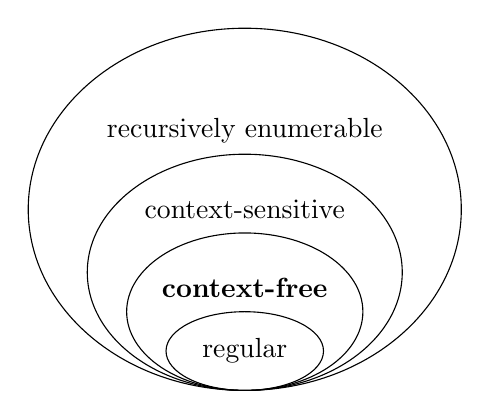
\begin{tikzpicture}
            \node[] at (2,2) {regular};
            \draw (2,2) ellipse (1cm and 0.5cm);
            \node[] at (2,2.8) {\textbf{context-free}};
            \draw (2,2.5) ellipse (1.5cm and 1cm);
            \node[] at (2,3.8) {context-sensitive};
            \draw (2,3) ellipse (2cm and 1.5cm);
            \node[] at (2,4.8) {recursively enumerable};
            \draw (2,3.8) ellipse (2.75cm and 2.3cm);
        \end{tikzpicture}
        \caption{\label{fig:3.2}Chomsky/Chomsky–Schützenberger Hierarchy}
    \end{center}
\end{figure}

\begin{enumerate}
    \item \textbf{Regular grammar}
    \begin{enumerate}
        \item Only single non-terminals can be on the left-hand side of production rules
        \item The right-hand side of production rules must follow either\dots
        \begin{itemize}
            \item A terminal symbol followed by zero or one non-terminal symbol \textbf{(right regular)}
            \item Zero or one non-terminal symbol followed by a terminal symbol \textbf{(left regular)}
        \end{itemize}
        \item An example of a regular grammar is shown in \hyperref[fig:3.1]{fig. 3.1} which is \textbf{right regular}
    \end{enumerate}
    \item \textbf{Context-free}: discussed in section \hyperref[sec:features-context-free]{3.1.3}
    \item \textbf{Context-sensitive}
    \begin{enumerate}
        \item Production rules are in the form:
        \begin{center}
            $\alpha A \beta \rightarrow \alpha \gamma \beta$
        \end{center}
        \item $S \rightarrow \epsilon$ can only exist if $S$ doesn't occur on the right-hand side of any production rule
        \item Where $A$ is a non-terminal and $\alpha$, $\beta$, and $\gamma$ are non-terminals or terminals, $\alpha$ and $\beta$ may be empty, and $\gamma$ must be non-empty.
        \item The English language is an example of a context-sensitive language
    \end{enumerate}
    \item \textbf{Recursively enumerable}: are all languages that can be recognisable by Turing machines and encompass all formal languages\textsuperscript{\cite{geuvers_rot_2016}}
\end{enumerate}

\pagebreak

\section{Manual Parsing Techniques}

When it comes to parsing algorithms they are split into two main groups: \textbf{top-down} parsers and \textbf{bottom-up} parsers. This relates to the way that the \textbf{parse tree} is constructed for a given input string.

A \textbf{parse tree} is a rooted tree that represents the syntactic structure of an input string. The grammar accepted by parsers that generate a parse tree must have a non-terminal root/start symbol which encompasses the entire input string as well as terminal symbols which form the leaf nodes of the tree. In other words, a context-free grammar.

Practically, parse trees can be passed into a semantic analyser to produce an Abstract Symbol Tree (AST), which can then be traversed to produce code in a compiled language or executed directly in an interpreted language.

\subsection{A note on derivations}

Given an input string $S$ and a grammar $G$, the derivation of $S$ on grammar $G$ is one of the possible sequences of grammar rules that must be applied to transform the start symbol into $S$. Thus, proving that the string $S$ belongs in the language defined by grammar $G$.

For instance, given the following grammar describes the syntax that could be accepted by a four function calculator:

% Grammar for four function calc
\begin{figure}[h]
    \begin{center}
        \begin{verbatim}
            E ::= T | E A
            A ::= "+" T | "-" T
            T ::= F | T P
            P ::= "*" F | "/" F
            F ::= N | (E)
            N ::= Z | N D
            Z ::= 1 | 2 | 3 | 4 | 5 | 6 | 7 | 8 | 9
            D ::= 0 | 1 | 2 | 3 | 4 | 5 | 6 | 7 | 8 | 9
        \end{verbatim}
    \end{center}
    \vspace{-1.5em}
    \caption{\label{fig:3.3}Grammar describing the syntax of a four function calculator}
\end{figure}

\pagebreak

One of the possible derivations for the string \verb|1 + 2 * 3| with the start state $E$ could be...

% Possible derivation of "1 + 2 * 3" with start symbol E
\begin{figure}[h]
    \begin{equation}
        \begin{split}
            E &\rightarrow EA\\
            &\rightarrow TA\\
            &\rightarrow FA\\
            &\rightarrow NA\\
            &\rightarrow ZA\\
            &\rightarrow 1 A\\
            &\rightarrow 1 + T\\
            &\rightarrow 1 + TP\\
            &\rightarrow 1 + FP\\
            &\rightarrow 1 + NP\\
            &\rightarrow 1 + ZP\\
            &\rightarrow 1 + 2 P\\
            &\rightarrow 1 + 2 * F\\
            &\rightarrow 1 + 2 * N\\
            &\rightarrow 1 + 2 * Z\\
            &\rightarrow 1 + 2 * 3
        \end{split}
        \nonumber
    \end{equation}
    \vspace{-1.5em}
    \cprotect\caption{\label{fig:3.4}A possible derivation of \verb|1 + 2 * 3| with start state $S$ on the grammar given in \hyperref[fig:3.3]{fig. 3.3}}
\end{figure}

This derivation is performed \textit{top-down} by taking the \textit{leftmost derivation}, this means that we start with the start state and produce a parse tree by applying the derivation step for the leftmost non-terminal until we end up with the input string. The grammar that is given in \hyperref[fig:3.3]{fig. 3.3} is \textbf{ambiguous}, which means that this derivation belongs to the set of all possible derivations. Each possible derivation can be treated as a different choice subtree whenever a production rule with no terminals on the right-hand side is used. This is the building block for \hyperref[sec:top-down]{recursive descent parsers with backtracking}.

\subsection{Top-down vs. Bottom-up parsing}

\subsubsection{Top-down}
\label{sec:top-down}

\begin{definition}[Top-down parser]
    A top-down parser produces a parse tree by starting at a given state $S$ by applying derivation steps until the input string is reached. Backtracking might be used in certain grammars to assure a correct derivation is reached.
\end{definition}

For a `human operated' derivation, the style shown in \hyperref[fig:3.4]{fig. 3.4} seems easier to digest. This is because as humans, we can lookahead in the input expression and decide which derivation step to apply. This makes manual parsing for a given grammar trivial, for example given the grammar:

\begin{figure}[h]
    \begin{center}
        \begin{verbatim}
            J ::= [] | {} | [ E ] | { K }
            E ::= J | E, J
            K ::= S: J | K, S: J
            S ::= " a | b | c "
            N ::= 0 | 1 | 2 | 3 | 4 | 5 | 6 | 7 | 8 | 9
        \end{verbatim}
    \end{center}
    \vspace{-1.75em}
    \caption{\label{fig:3.5}Grammar for a reduced JSON-like metalanguage}
\end{figure}

The top-down parse tree for the input string: \verb|{"a": 0}|, can be constructed manually very easily.

\begin{figure}[h]
    \begin{center}
        \begin{forest}
            for tree={
                if n children=0{
                  font=\itshape,
                }{},
              }
              [$J_1$
                [{\{}]
                [$K_2$
                  [$S_3$
                    [{"}]
                    [$a$]
                    [{"}]
                  ]
                  [{:}]
                  [$J_4$
                    [$N_5$
                        [$0$]
                    ]
                  ]
                ]
                [{\}}]
              ]
        \end{forest}
    \end{center}
    \vspace{-1.75em}
    \cprotect\caption{\label{fig:3.6}The parse/derivation tree produced by the top-down parsing of the string \verb|{"a": 0}|}
\end{figure}

However, when it comes to creating a formal algorithm definition for this technique, it becomes a lot less straightforward. This is because at every non-terminal symbol the parser has to explore each possible derivation step. Effectively building multiple subtrees below it and finally choosing the one which ends up at the correct terminal, or backtracking to the previous derivation step if no match can be found.

There are ways to optimise top-down parsing such as restructuring the grammar to be accepted by an LL(1) parser. The grammar in \hyperref[fig:3.7]{fig. 3.7} is the grammar in \hyperref[fig:3.6]{fig. 3.6} restructured to remove all left-recursion.

\begin{definition}[Left-recursive grammars]
    A grammar is left-recursive if it has a non-terminal $A$ such that there is a derivation sequence $A \stackrel{\mathclap{\normalfont\mbox{+}}}{\Rightarrow} A \alpha$ for some string $\alpha$. Left recursion causes recursive descent to fall into an infinite loop due to the parse tree being constructed in a depth-first leftmost fashion.\textsuperscript{\cite{scott_johnstone_1998}}
\end{definition}

\begin{figure}[h]
    \begin{center}
        \begin{equation}
            \begin{split}
                J &\rightarrow O\;|\;A\\
                O &\rightarrow [\;]\;|\;[\;M\;]\\
                M &\rightarrow P\;|\;P\;,\;M\\
                P &\rightarrow S\;:\;V\\
                A &\rightarrow [\;]\;|\;[\;E\;]\\
                E &\rightarrow V\;|\;V,\;E\\
                V &\rightarrow	S\;|\;N\\
                S &\rightarrow	"a"\;|\;"b"\;|\;"c"\\
                N &\rightarrow 0\;|\;1\;|\;2\;|\;3\;|\;4\;|\;5\;|\;6\;|\;7\;|\;8\;|\;9
            \end{split}
            \nonumber
        \end{equation}
    \end{center}
    \vspace{-1em}
    \caption{\label{fig:3.7}The grammar in \hyperref[fig:3.6]{fig. 3.6} restructured to remove left-recursion}
\end{figure}

\begin{definition}[First-set]
    The first set for a non-terminal consists of all the terminals that can be found by following each of its production rules until a rule beginning with a terminal is found.
\end{definition}

\begin{figure}[H]
    \begin{center}
        \begin{equation}
            \begin{split}
                J &= \{``\{", ``\}"\}\;
                O = \{ ``\{" \}\;
                M = \{ \text{``"'} \}\;
                P = \{ \text{``"'} \}\;
                A = \{ ``[" \}\\
                E &= \{ \text{``"'}, ``0", ``1", ``2", ``3", ``4", ``5", ``6", ``7", ``8", ``9" \}\\
                V &= \{ \text{``"'}, ``0", ``1", ``2", ``3", ``4", ``5", ``6", ``7", ``8", ``9" \}\\
                S &= \{ ``\{" \}\\
                N &= \{``0", ``1", ``2", ``3", ``4", ``5", ``6", ``7", ``8", ``9" \}
            \end{split}
            \nonumber
        \end{equation}
    \end{center}
    \caption{\label{fig:3.8}First-sets of each terminal and non-terminal}
\end{figure}

However, this grammar is still not LL(1) due to the first set conflicts within $O$, $M$, $E$, $A$, and $S$. This occurs when the first sets of two different production rules for the same non-terminal intersect with each other. After left factoring the grammar, it is now acceptable by an LL(1) parser.

\begin{figure}[H]
    \begin{center}
        \begin{equation}
            \begin{split}
                J &\rightarrow	O\;|\;A\\
                O &\rightarrow	\{\;Fcurly\\
                Fcurly &\rightarrow\;\}\;|\;M\;\}\\
                M &\rightarrow	P\;\;FP\\
                FP &\rightarrow\;\epsilon\;|\;,\;M\\
                P &\rightarrow	S\;:\;V\\
                A &\rightarrow	[\;Fsqr\\
                Fsqr &\rightarrow \;]\;|\;E\;]\\
                E &\rightarrow	V\;\;FV\\
                FV &\rightarrow\;\epsilon\;|\;,\;E\\
                V &\rightarrow	S\;|\;N\\
                S &\rightarrow	"\;Fquote\\
                Fquote &\rightarrow\;a\;"\;|\;b\;"\;|\;c\;"\\
                N &\rightarrow	0\;|\;1\;|\;2\;|\;3\;|\;4\;|\;5\;|\;6\;|\;7\;|\;8\;|\;9
            \end{split}
            \nonumber
        \end{equation}
    \end{center}
    \vspace{-1em}
    \caption{\label{fig:3.9}Grammar in \hyperref[fig:3.7]{fig. 3.7} restructured to remove first-set conflicts using the removal of left factors method}
\end{figure}

\pagebreak

We can now construct a unique top-down derivation of \verb|{"a": 0}|:

\begin{figure}[H]
    \begin{center}
        \begin{forest}
            for tree={
                if n children=0{
                  font=\itshape,
                }{},
              }
              [$J_1$
                [$O$
                    [{\{}]
                    [Fcurly
                        [M
                            [P
                                [S
                                    ["]
                                    [Fquote
                                        [a"]
                                    ]
                                ]
                                [:]
                                [V
                                    [N
                                        [0]
                                    ]
                                ]
                            ]
                            [FP
                                [$\epsilon$]
                            ]
                        ]
                        [{\}}]
                    ]
                ]
              ]
        \end{forest}
    \end{center}
    \cprotect\caption{\label{fig:3.10}The unique derivation of \verb|{"a": 0}| after restructuring the grammar in \hyperref[fig:3.5]{fig. 3.5} to be an LL(1) grammar}
\end{figure}

As you can see this is quite an involved process which results in a grammar that is very different to the grammar that was specified in \hyperref[fig:3.5]{fig. 3.5}. This confusing grammar and the difficulty of construction is often why top-down parser generators are avoided when defining the grammar for a programming language.
    
\subsubsection{Bottom-up}

\begin{definition}[Bottom-up parser]
    A bottom-up parser produces a parse tree by starting at a given input string and applying derivation steps until the start symbol of the grammar is reached. Effectively constructing the derivation tree from the leaf nodes upwards. Shift-reduce parsers are an example of bottom up parsing and have a linear runtime.
\end{definition}

% Describe the shift-reduce algorithm and give an example

Even though it seems unnatural to construct a derivation tree from the bottom-up there is one method that is quite intuitive for manual use. This is shift-reduce parsing. We shall define a new grammar (\hyperref[fig:3.11]{fig. 3.11}) for the upcoming example of the shift-reduce method.

\begin{figure}[h]
    \begin{center}
        \begin{equation}
            \begin{split}
                Section &::= Header\;Property\;|\;Section\;Property\;|\;Section\;Header\\
                Header &::= [\;S\;]\\
                Property &::= S\;=\;V;\\
                V &::= S\;|\;N\\
                S &::= a\;|\;b\;|\;c\\
                N &::= 0\;|\;1\;|\;2\;|\;3\;|\;4\;|\;5\;|\;6\;|\;7\;|\;8\;|\;9
            \end{split}
            \nonumber
        \end{equation}
    \end{center}
    \vspace{-1em}
    \caption{\label{fig:3.11}Grammar for a simplified INI config file type language}
\end{figure}

\pagebreak

Shift-reduce parsing parses a given input string by applying one of the two actions:

\begin{itemize}
    \item \textbf{Reduce}: If we can find a rule $A \rightarrow \alpha$ and if the contents of the stack are $\beta\alpha$ for some $\beta$, then we can reduce the stack to $\beta A$. In effect, we are applying production rules for non-terminals backwards. If the \textbf{current stack is just the start symbol} and \textbf{no input is left}, then this means that the given input is a valid sentence within the language defined by the given grammar.
    \item \textbf{Shift}: If it's not possible to perform a reduction on the current stack symbol, then the next terminal can be pushed onto the stack from the input.
\end{itemize}

Along with those actions we also define a \textbf{lookahead} variable which defines the next available token in the input. This is necessary to parse the grammar in \hyperref[fig:3.11]{fig. 3.11}. For example, if the symbol $S$ was on the stack we might need to use the lookahead to see if the next token is ``$]$" or ``$=$" to avoid reducing $S$ into $V$.\textsuperscript{\cite{johnson_zelenski_2007}\cite{knuth_1965}}

Different amounts of lookahead denote different subsets of grammars. For instance, the grammar defined in \hyperref[fig:3.11]{fig. 3.11} is an $LR(1)$ grammar, where there is $1$ token of lookahead.

With that in mind here's an example of a shift-reduce trace table using the grammar given in \hyperref[fig:3.11]{fig. 3.11}:

\begin{figure}[H]
    \begin{center}
        \begin{tabular}{| m{3.5cm} | m{3cm} | m{2cm} | m{5cm} |}
            \hline
            Stack & \mbox{Remaining Input} & Lookahead & Action\\
            \hline
            & \verb|[a]a=0;b=a;$| & \verb|[| & Shift\\
            \hline
            \verb|[| & \verb|a]a=0;b=a;$| & \verb|a| & Shift\\
            \hline
            \verb|[a| & \verb|]a=0;b=a;$| & \verb|]| & Reduce: $S \rightarrow a$\\
            \hline
            \verb|[S| & \verb|]a=0;b=a;$| & \verb|]| & Lookahead is \verb|]|. Longest match.\\
            \hline
            \verb|[S]| & \verb|a=0;b=a;$| & \verb|a| & Reduce: $Header \rightarrow [\;S\;]$\\
            \hline
            \verb|Header| & \verb|a=0;b=a;$| & \verb|a| & Shift\\
            \hline
            \verb|Header a| & \verb|=0;b=a;$| & \verb|=| & Reduce: $S \rightarrow a$\\
            \hline
            \verb|Header S| & \verb|=0;b=a;$| & \verb|=| & Lookahead is \verb|=|. Longest match.\\
            \hline
            \verb|[Header S=| & \verb|0;b=a;$| & \verb|0| & Shift\\
            \hline
            \verb|Header S=0| & \verb|;b=c;$| & \verb|;| & Reduce: $N \rightarrow 0$\\
            \hline
            \verb|Header S=N| & \verb|;b=c;$| & \verb|;| & Reduce: $V \rightarrow N$\\
            \hline
            \verb|Header S=V| & \verb|;b=c;$| & \verb|;| & Shift\\
            \hline
            \verb|Header S=V;| & \verb|b=c;$| & \verb|b| & Reduce: $Property \rightarrow S = V;$\\
            \hline
            \verb|Header Property| & \verb|b=c;$| & \verb|b| & Reduce: $Section \rightarrow Header\;Property$\\
            \hline
            \verb|Section| & \verb|b=c;$| & \verb|b| & Shift\\
            \hline
            \verb|Section b| & \verb|=c$;| & \verb|=| & Reduce: $S \rightarrow b$\\
            \hline
            \verb|Section S| & \verb|=c;$| & \verb|=| & Lookahead is \verb|=|. Longest match.\\
            \hline
            \verb|Section S=| & \verb|c;$| & \verb|c| & Shift\\
            \hline
            \verb|Section S=c| & \verb|;$| & \verb|;| & Reduce: $S \rightarrow c$\\
            \hline
            \verb|Section S=S| & \verb|;$| & \verb|;| & Reduce: $V \rightarrow S$, lookahead is ``$;$": assume that reduction to $V$ can be made.\\
            \hline
            \verb|Section S=V| & \verb|;$| & \verb|;| & Shift\\
            \hline
            \verb|Section S=V;| & \verb|$| & \verb|$| & Reduce: $Property \rightarrow S = V;$\\
            \hline
            \verb|Section Property| & \verb|$| & \verb|$| & Reduce: $Section \rightarrow Section\;Property$\\
            \hline
            \verb|Section| & \verb|$| & \verb|$| & \\
            \hline
        \end{tabular}
    \end{center}
    \cprotect\caption{\label{fig:3.12}Trace table for a shift-reduce parser with the input \verb|[a]a=0;b=a;| with the grammar shown in \hyperref[fig:3.11]{fig. 3.11}}
\end{figure}

As you can see if the grammar is LR(1), a shift-reduce method can easily be carried out manually. This is because, as a human, you can look back at the production rules given in the grammar and apply the reductions/shifts appropriately.

Algorithms for shift-reduce parsing involve \textbf{lookup tables} that contain the action to carry out for each symbol that can lie at the top of the stack, as well as the next input symbol which can be read in. Most LR based parsers involve constructing a deterministic finite-state automaton which is then converted to a parse table for efficiency.\textsuperscript{\cite{hopcroft_motwani_ullman_2006}}

It is also worth noting that in \hyperref[fig:3.12]{fig. 3.12}, when the action taken includes the `longest match' phrase. This means that the shift will be taken over the reduction that can be made in the parser's current state. This functionality is included in many parser generators/compiler compilers such as YACC.

\section{Parser generators}

The parser generator that I will be using for my interpreter is the \href{https://github.com/alecthomas/participle#overview}{participle parser by Alec Thomas}. Participle will generate a recursive descent parser with backtracking for a given grammar. This means that the grammar you need to write can be, but is not limited to LL(1). However, if the grammar is not LL(1) the parser is not guaranteed to terminate. This means that grammar will need to be restructured to remove any left-recursion (if it exists). If the grammar is \textbf{not} left recursive then backtracking still might need to be used by the parser if the grammar is not left-factored or not follow determined.

If a grammar that is LL(1) can be constructed it will mean that the parser generated will be a \textit{predictive parser} which means that there will be no backtracking.
